\subsection{Description du déroulement projet}

Dans cette section, nous allons retracer le déroulement du projet au travers de l'analyse des burndown charts de chacun des sprints.

\subsubsection{Sprint 1}

\begin{figure}[h]
\begin{center}
	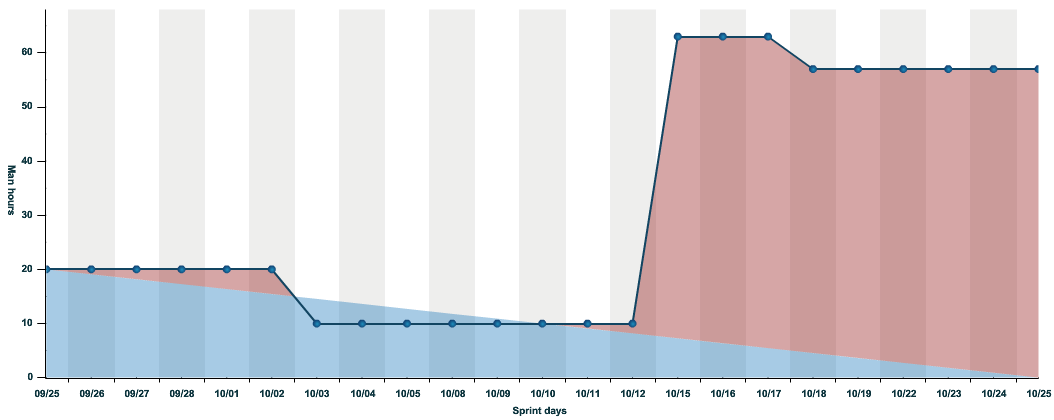
\includegraphics[width=11cm]{burndown-S1.png}
\end{center}
	\caption{Burdown chart du sprint 1}
\end{figure}

L'activité principale de ce premier sprint a été de créer une couche modèle pour notre application. Ceci impliquait de trouver une bibliothèque permettant de lire le format dicom et qui soit compatible avec android. Cette tache a demandé beaucoup d'investissement et de recherche et n'a pu être achevée qu'au sprint suivant. C'est pourquoi on remarque trois plateaux de stagnation. L'augmentation spectaculaire du nombre d'homme-heure restant vers la fin du sprint est du à une mauvaise utilisation de l'outil. En effet, ce sprint nous a introduit à la méthode \emph{scrum} et aux outils associés. De ce fait, notre manque d'assurance et de maîtrise explique les imperfections de ce sprint. Néanmoins, on constate tout de même que des avancées significatives ont pu être réalisées durant ce sprint, la partie modèle étant en majorité achevée lors du passage au deuxième sprint.

\subsubsection{Sprint 2}

\begin{figure}[h]
\begin{center}
	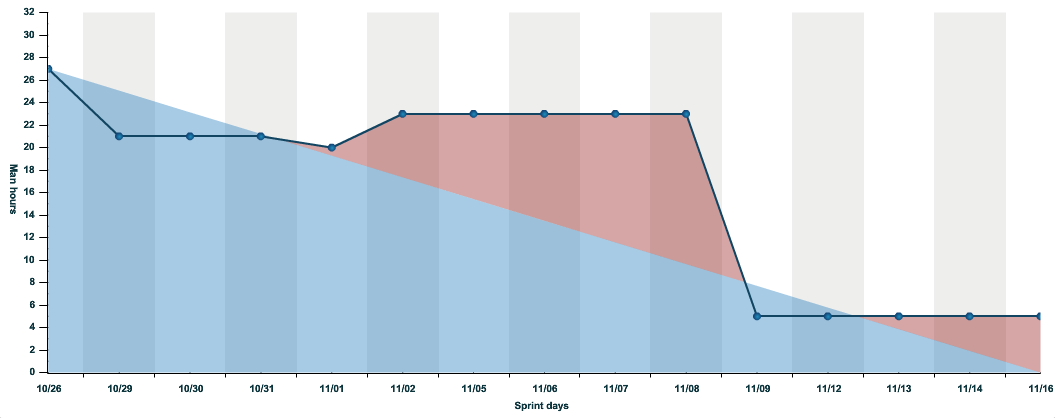
\includegraphics[width=11cm]{burndown-S2.png}
\end{center}
	\caption{Burndown chart du sprint 2}
\end{figure}

Après la prise en main de la méthode \emph{scrum} et des outils au cours du premier sprint, nous avons pu aborder ce deuxième sprint plus en confiance. On constate un bon départ, les tâches les plus faciles ayant été réalisées en premier. Des tâches plus ardues ont ralenti la progression vers le milieu du sprint, mais nous avons su travailler de concert pour surmonter les difficultés et revenir en deçà de la prévision. Les quelques tâches inachevées ont été reportées au dernier sprint. Globalement, ce deuxième sprint est très positif, notre première expérience en \emph{scrum} nous permettant de mieux gérer l'évaluation et la répartition des tâches. Le seul point négatif est la présence de tâches inachevées, c'est pourquoi nous avons décider de revoir notre capacité de travail à la baisse pour le sprint final.

\subsubsection{Sprint 3}

\begin{figure}[h]
\begin{center}
	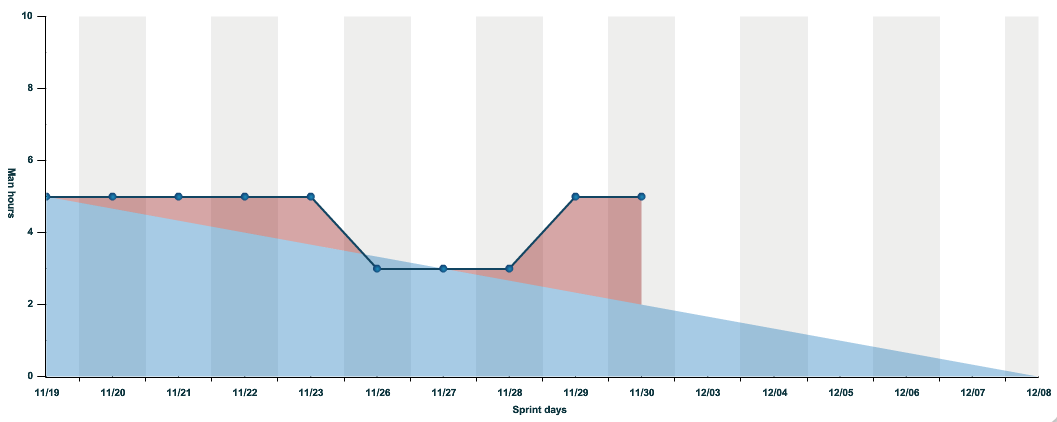
\includegraphics[width=11cm]{burndown-S3.png}
\end{center}
	\caption{Burndown chart du sprint 3}
\end{figure}

Les quelques difficultés rencontrées en début de sprint 3 ont pu être surmontées grâce au concours de toute l'équipe. Les tâches restantes en fin de sprint 2 et les tâches simples du sprint 3 ont été rapidement réalisées. On peut remarquer une augmentation du travail à réaliser. Ceci est du à la modification d'un besoin par le client et son intégration au sprint. Malheureusement, ce sprint n'a pas pu être mené à son terme à cause des impératifs calendaires de rendu.
%partie à modifier en fonction de l'issue du BMI3D